\chapter{行走} \label{chap:chap2}

\begin{figure}[!htb]
	\centering
	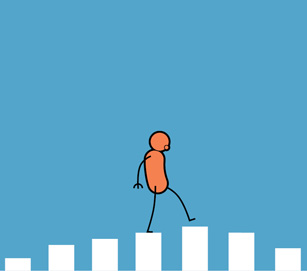
\includegraphics[width=0.5\linewidth]{chap2/2_0}
	% 加星号(*)表示不加编号
	\caption*{ \label{fig:2_0}}
\end{figure}

每走一步,你都会向前倾斜一点点,然后站稳,避免摔倒,一遍又一遍,你都在摔倒,然后站稳,避免摔倒。

\begin{flushright}
	——劳里·安德森 \\
\end{flushright}

\begin{figure}[!htb]
	\centering
	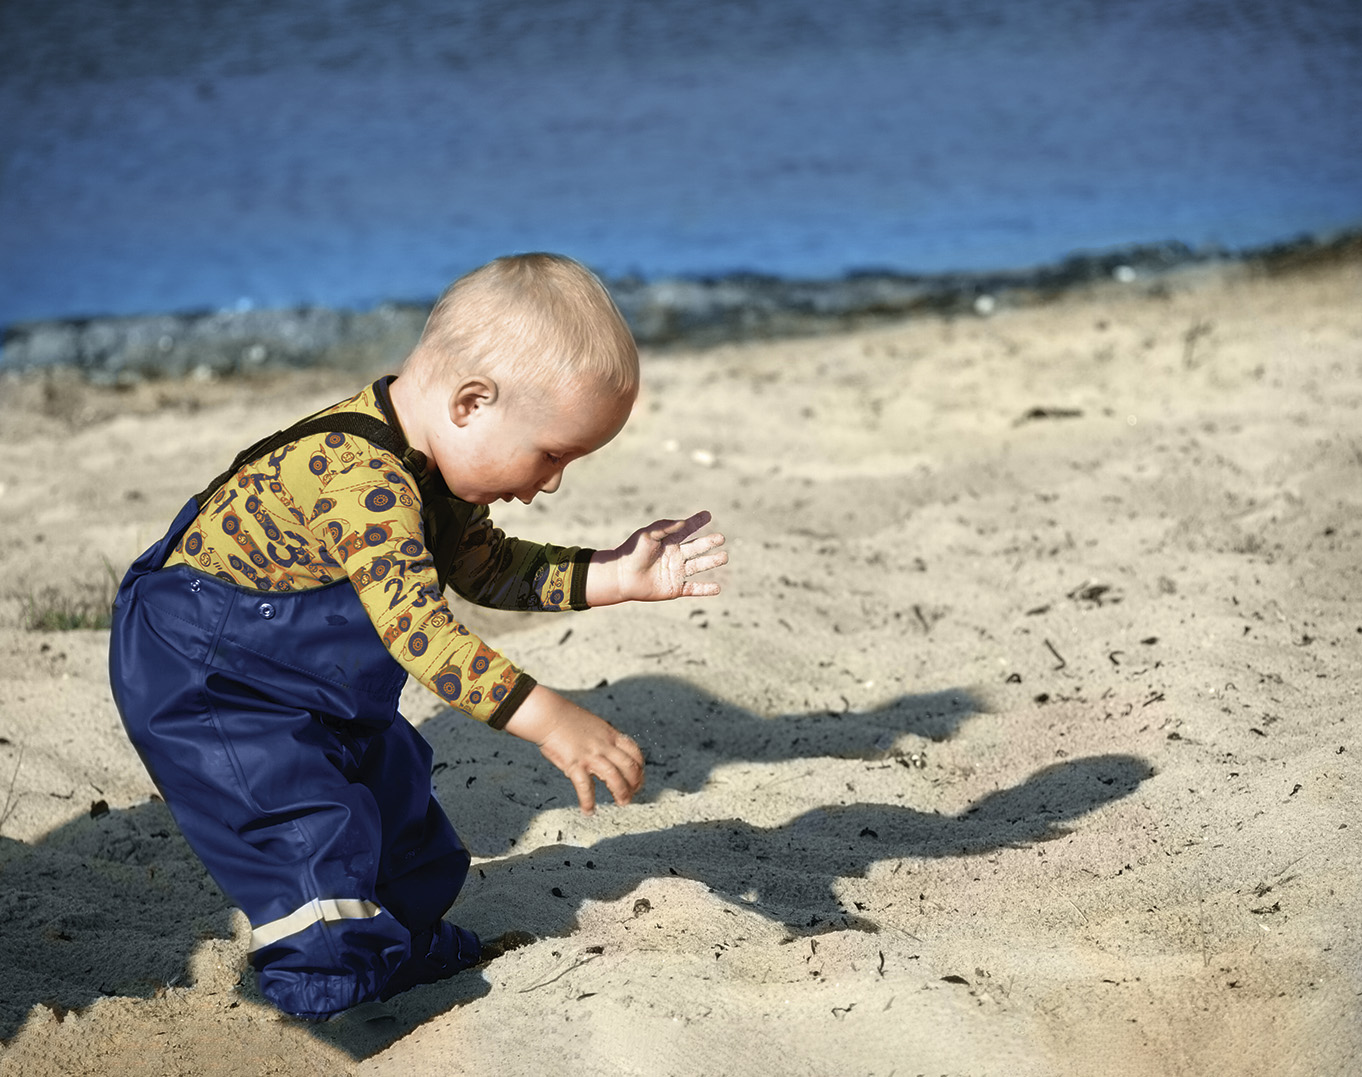
\includegraphics[width=0.5\linewidth]{chap2/2_0_2}
	% 加星号(*)表示不加编号
	\caption*{ \label{fig:2_0_2}}
\end{figure}

“有一天,我在月球上漫步,”
宇航员哈里森$\cdot$施密特兴高采烈地唱着,他即将踏上最后一次阿波罗任务的首次月球行走。
“在快乐的五月,”指挥官吉恩$\cdot$塞尔南附和道。
一缕缕月尘从他们的靴子上溅起,他们……究竟在做什么?跳跃?腾跃?跌跌撞撞?……穿过月球表面。


不管它是什么,它与我们通常认为的行走几乎没有什么相似之处。
施密特像个蹒跚学步的孩子一样慢步走着,左右摇晃。
塞尔南的步态看起来像个孩子骑着扫帚,却假装那是一匹马。
这两位训练有素的宇航员仿佛忘记了人类最基本的技能——行走——不得不学习一种新的移动方式(图~\ref{fig:2_1})。


\begin{figure}[!htb]
	\centering
	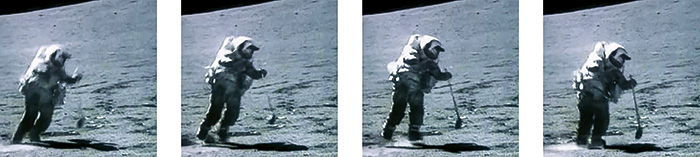
\includegraphics[width=1.0\linewidth]{chap2/2_1}
	\caption{宇航员很少在月球表面“行走”,他们更喜欢在月球引力下跳跃行走。
		图片由NASA提供。 \label{fig:2_1}}
\end{figure}


在本章中,我们将探讨为何看似简单的行走——人类进化已完美适应地球引力——在月球上却变得如此困难。
宇航员奇特的步态或许能帮助我们更充分地理解行走过程中发生的一系列精心安排的事件,以及引力在其中扮演的关键角色。


欣赏行走壮举的另一种方式是建造一台能够行走的机器。
塔德$\cdot$麦吉尔(Tad McGeer)的巧妙实验表明,一个拥有类似人类比例的无动力装置可以在倾斜的表面上行走。
这些装置无需大脑、脊髓或肌肉即可行走,只需在正确的方向上轻轻推一下即可。
这一观察表明,我们可以通过简单的机械模型来深入了解行走,我们将在本章中对此进行演示。


然而,在开始分析之前,有必要先了解一下步态周期以及运动中涉及的一些基本物理知识。
下一节将为你提供一些正确的方向。


\section{步行步态周期}

人类有两种常见的步态:行走和跑步。
我们都熟悉身体各部分在行走时所经历的典型周期性模式,但更正式地描述这些定性观察结果会很有帮助。
一个行走步态周期由同一条腿上连续两次的足部接触事件界定,另一条腿的足部接触通常发生在中途(图~\ref{fig:2_2})。
每条腿都有一个支撑期(此时足部接触地面)和一个摆动期(此时足部离地)。
支撑期始于足部接触地面,结束于足尖离地,对于一条腿而言,它占行走步态周期的约 60\%;其余时间则用于摆动。
由于支撑期比摆动期长,因此在每个行走步态周期中,都有双脚接触地面的时期,我们称之为双支撑期。
我们将只有一只脚接触地面的间隔称为单支撑期。


\begin{figure}[!htb]
	\centering
	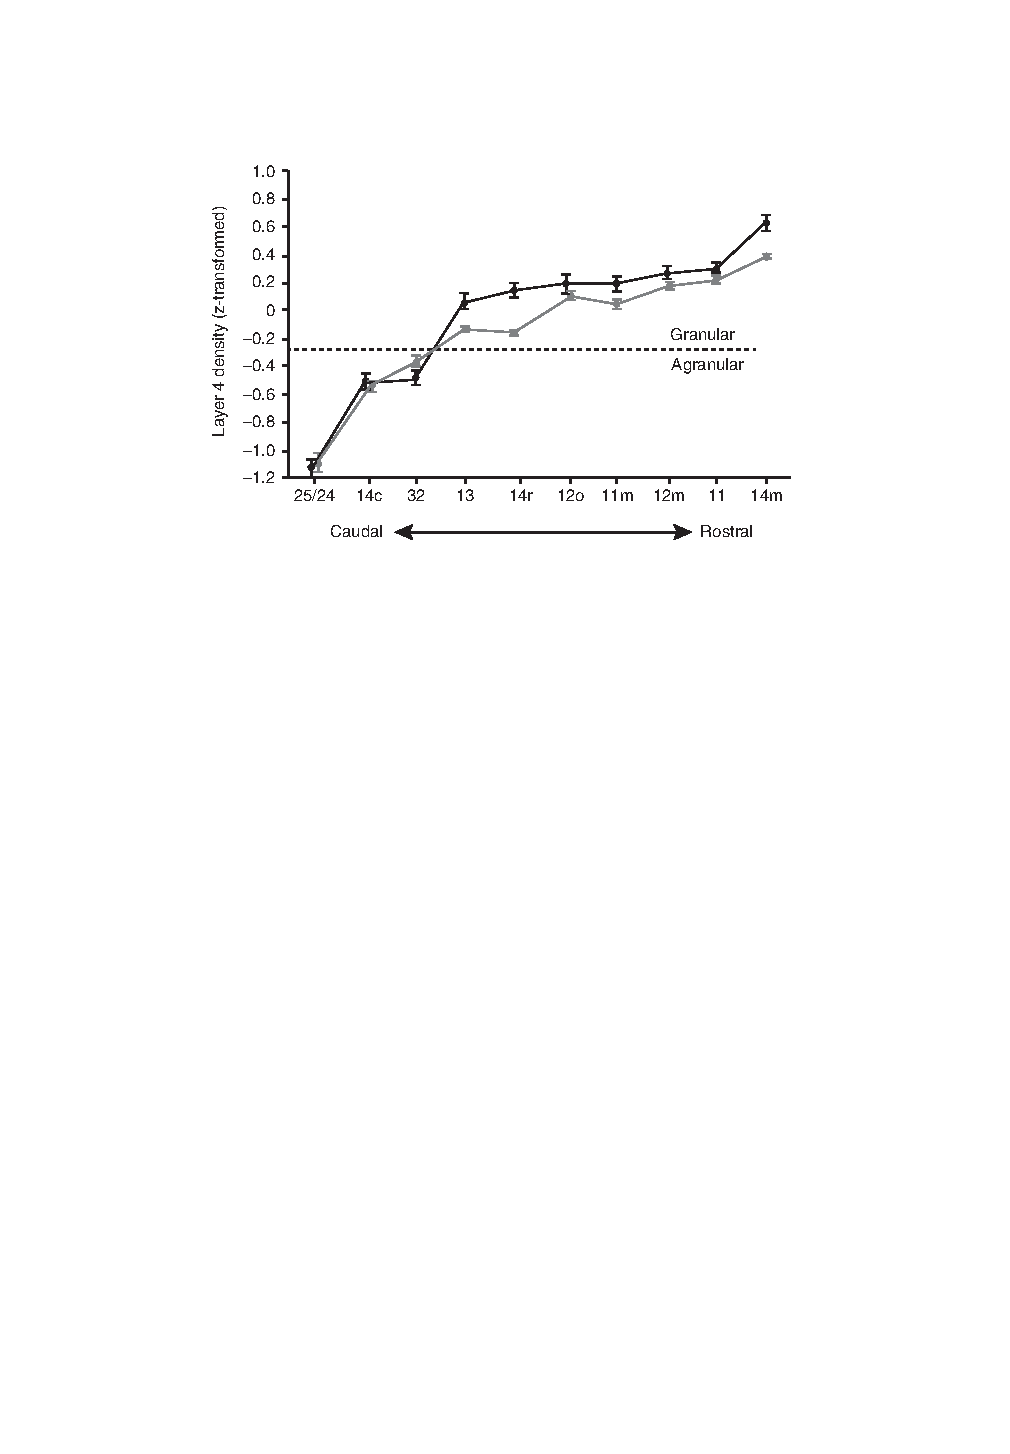
\includegraphics[width=1.0\linewidth]{chap2/2_2}
	\caption{步行步态周期及其组成事件(例如,脚接触)和阶段(例如,双支撑)。 \label{fig:2_2}}
\end{figure}


步长是指两个连续足迹上同一点之间沿行进线的距离(图~\ref{fig:2_3})。
连续两步所走的距离,或一个步态周期所走过的距离,称为步长。足部接触事件发生的速率(相当于步长持续时间的倒数)称为步频或步频;
迈步的速率称为步频。
步行速度可以用步长与步频的乘积来计算,或者也可以用步长与步频的乘积来计算:


\begin{figure}[!htb]
	\centering
	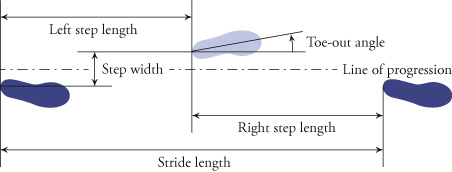
\includegraphics[width=0.8\linewidth]{chap2/2_3}
	\caption{水平(地面)平面上的步态测量。 \label{fig:2_3}}
\end{figure}

\begin{equation}
	\text{速度} = \text{步长} \times \text{步频}
			    = \text{步长} \times \text{起落}
\end{equation}

个人通常的步行速度会因身高、体能和其他因素而异。
健康成年人在平地上通常选择以约1.2-1.4米/秒的速度行走,步频为2步/秒。
典型的步长约为0.6-0.7米。


另外两个值得注意的指标是在水平面上测量的(图~\ref{fig:2_3})。
步宽是脚平放时脚后跟中点与另一条腿上相同点之间的距离,垂直于进展线测量。健康成年人的步宽约为腿长的 10\%。
如果腿长约为 1 米,步宽约为 10 厘米,但对于正在学习走路的幼儿和一些平衡能力较差的人来说,步宽会更大。
足部进展角是进展线与连接脚后跟中点和第二个脚趾(即足部的长轴)的线之间的角度。
正和负的足部进展角分别称为外倾角和内倾角。
成年人的外倾度通常较小,约为 10 度,但这个值在患有肌肉骨骼或神经系统疾病的个体之间可能会有所不同。
例如,患有小脑性共济失调(会导致平衡障碍)的人可能会以更大的脚趾向外和步宽行走,以减少跌倒的风险。


\section{地面反作用力}

我们通过测量双脚与地面之间的力来研究行走(图~\ref{fig:2_4})。
我们将在第~\ref{chap:chap11}~章中学习更多关于行走过程中肌肉协调的知识;
目前,只需知道肌肉通过产生力来产生运动即可。
肌肉产生的“作用力”会导致地面对双脚施加“反作用力”。
行走过程中,可以使用测力板测量地面反作用力。
测力板是一种仪器,可以测量人在测力板上行走时在垂直方向、前后方向和左右方向受到的力。​​
地面反作用力很重要,因为它可以衡量身体重心在每个时刻的加速度。
我们可以使用牛顿第二定律将地面反作用力和其他外力与身体重心 (com) 的加速度联系起来:
\begin{equation}
	F_{\text{external}} - mg = m a_{\text{com}} \label{eq:2_2}
\end{equation}
其中 $F_{external}$ 是施加于身体的所有外力之和,$m$ 是身体的总质量,$g$ 是重力加速度,$a_{com}$ 是质心加速度。
值得花点时间思考一下上一句中“和”和“全部”这两个词的含义。
当双脚接触地面时,我们必须将施加于每只脚的力相加。由于公式~\ref{eq:2_2}~是矢量和,所以方向很重要。
双脚下方力的垂直分量支撑着身体的重量。
但是,正如您在图~\ref{fig:2_5}~中所看到的,前脚上的前后力往往会抵消后脚上的前后力;
也就是说,前脚充当了刹车的作用,阻止我们走得越来越快,而后脚则提供推进力。
如果没有施加外力(即 $F_{external} = 0$,则物体处于自由落体状态,其质心将以 $g = 9.81 m/s^2$ 的速度加速向地面坠落。



\begin{figure}[!htb]
	\centering
	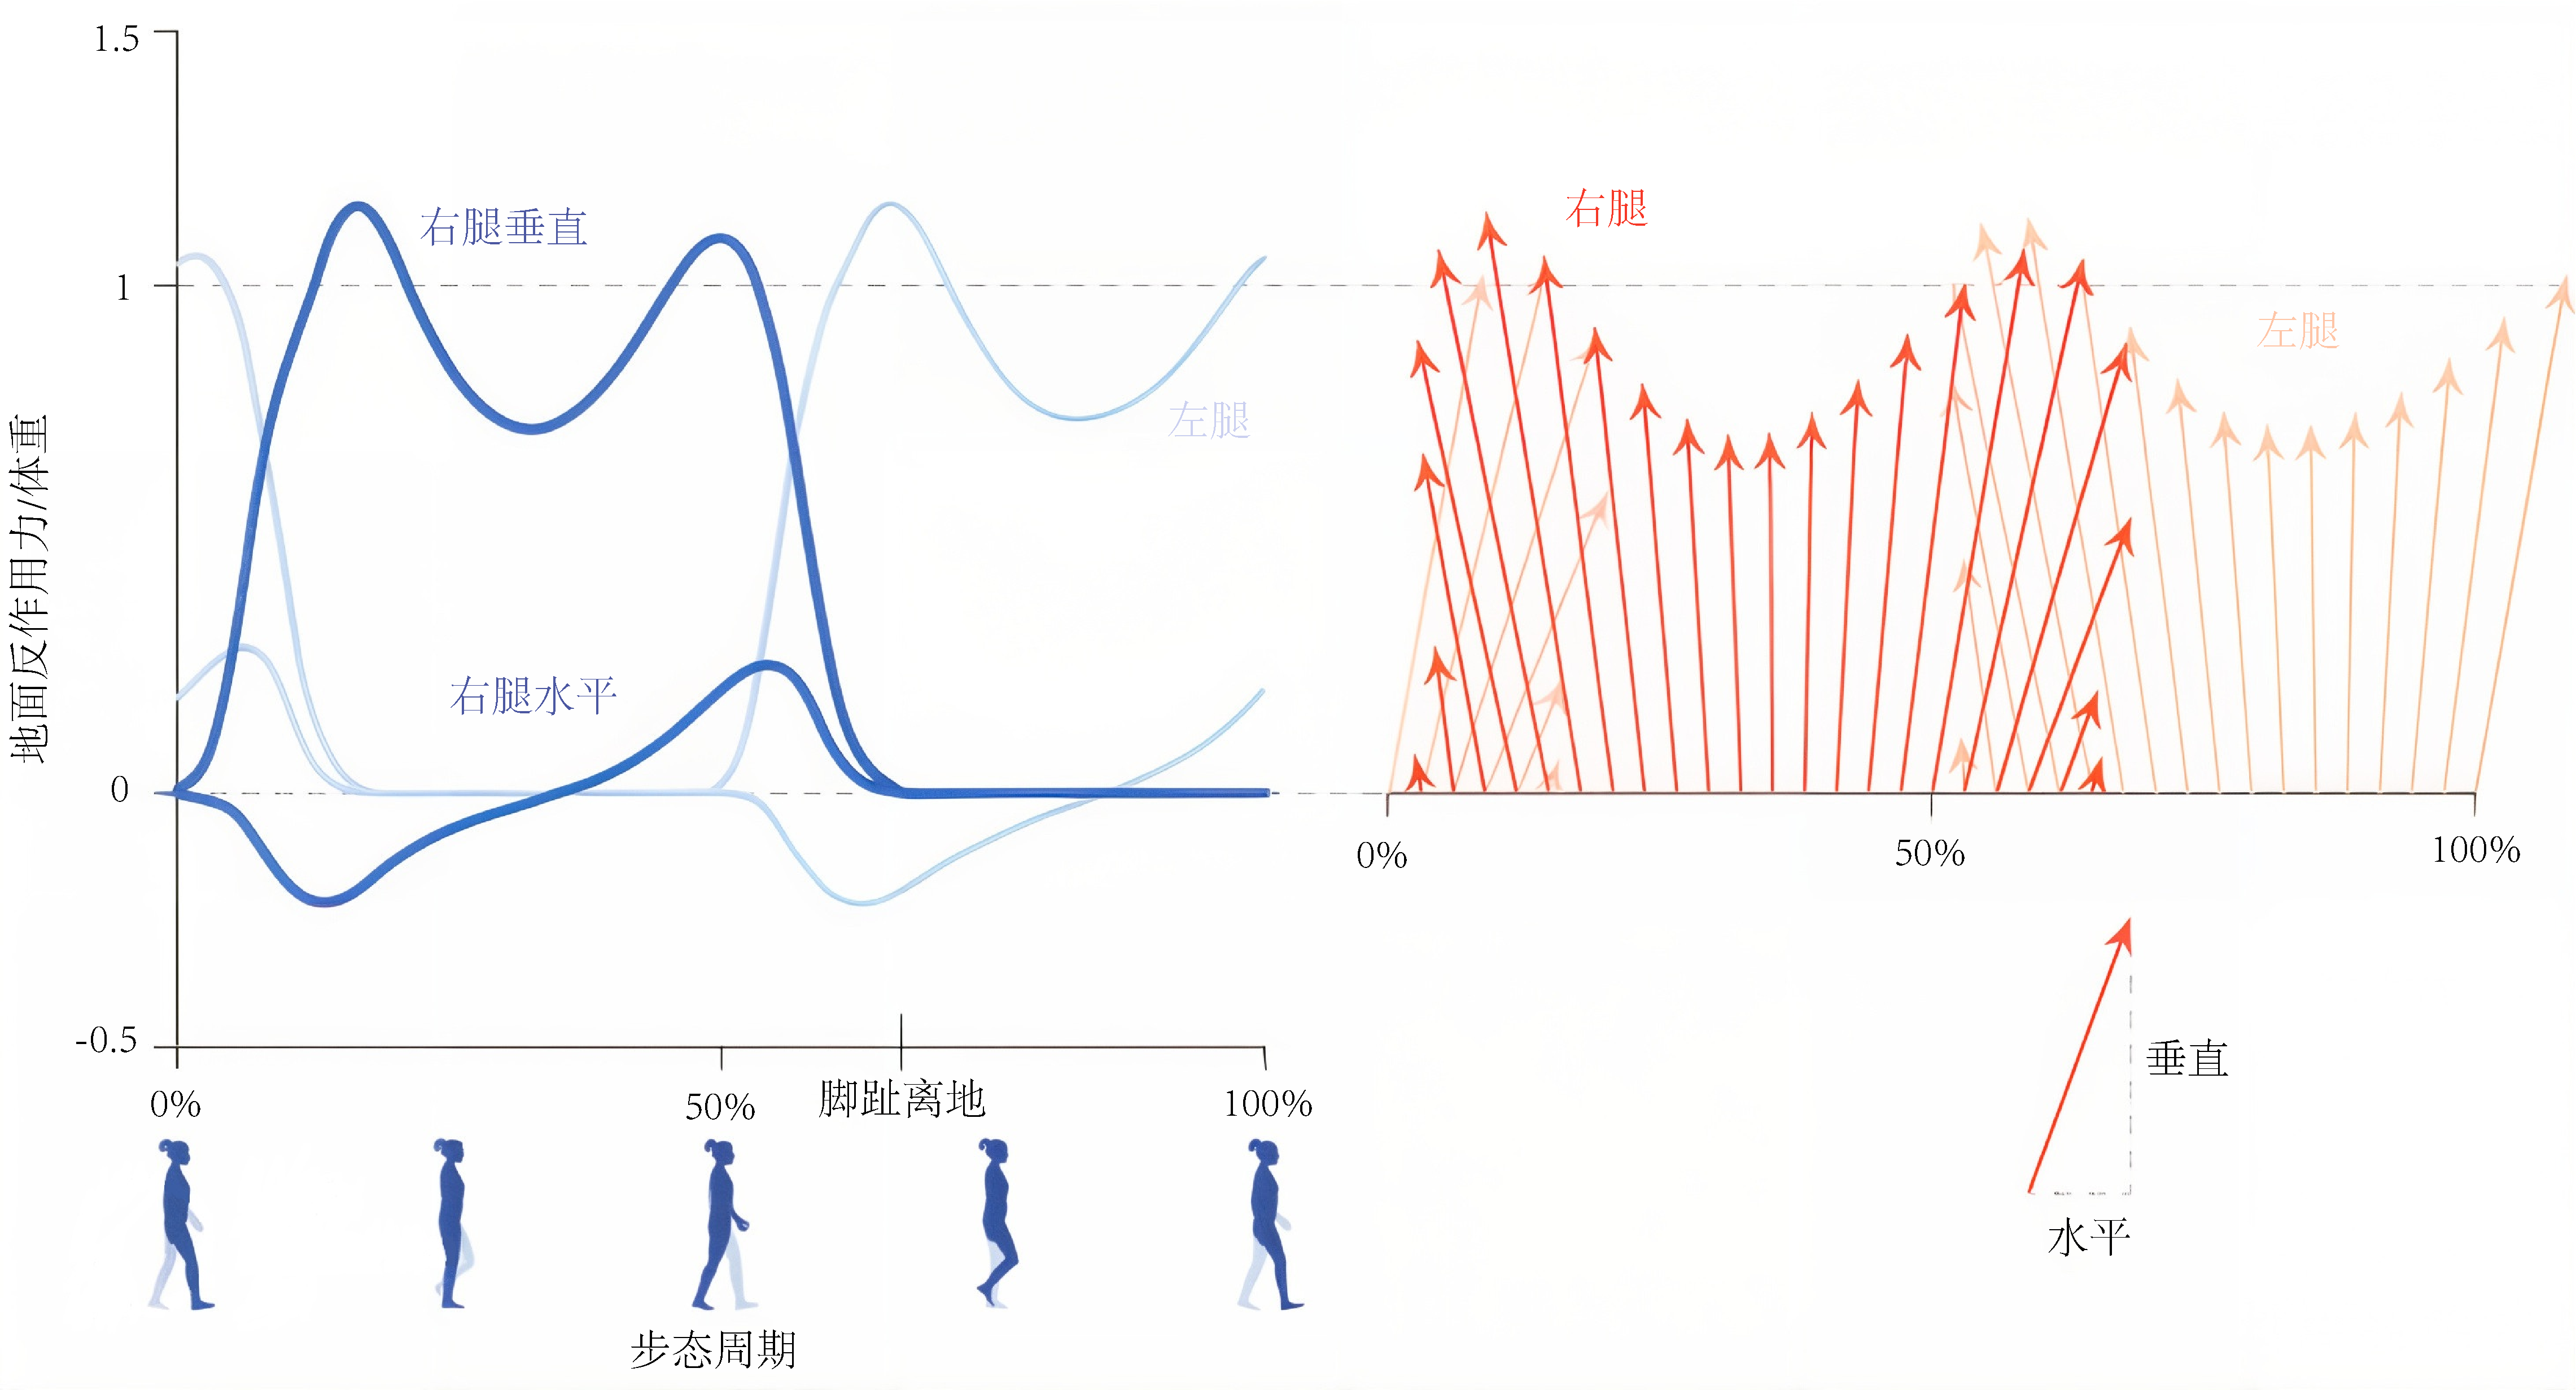
\includegraphics[width=1.0\linewidth]{chap2/2_4}
	\caption{以 1.55 米/秒的速度行走时代表性的地面反作用力。
		图中显示了步态周期内的垂直和水平(前后)分量(左)以及总矢量示意图(右)。
		正水平力指向前方。
		较小的左右力未显示。
		数据来自 Dembia 等人(2017)。 \label{fig:2_4}}
\end{figure}


\begin{figure}[!htb]
	\centering
	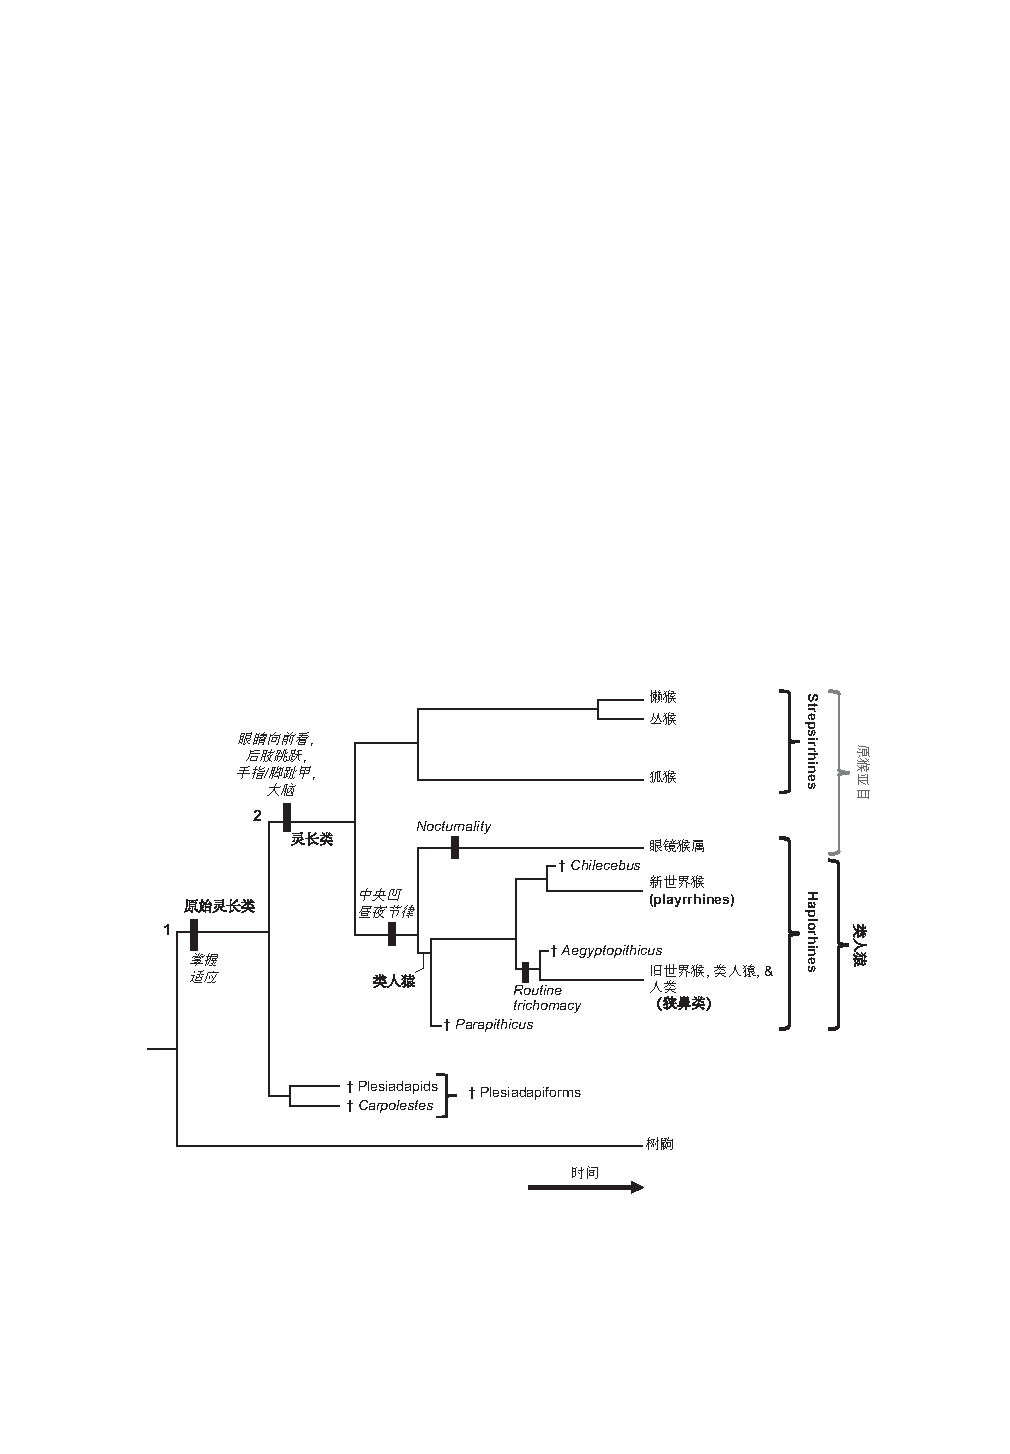
\includegraphics[width=0.9\linewidth]{chap2/2_5}
	\caption{以 1.55 米/秒的速度行走时,用两块测力板测量地面反作用力。
		两组箭头表示每只脚随时间推移受到的力。​​
		如黑色箭头所示,在双脚支撑时,地面反作用力的前后分量指向相反的方向。 \label{fig:2_5}}
\end{figure}


行走过程中地面反作用力的记录显示出几个有趣的特征(图~\ref{fig:2_6})。
地面反作用力的垂直分量在足部接触地面后迅速上升,并在步态周期的约 10\% 处达到大于体重的力。
在站立中期,垂直力降至低于体重,然后在蹬地时再次上升至高于体重。
然后,垂直力降至零,因为在脚趾离地后,足部不再接触地面。
平均而言,总垂直地面反作用力等于体重的 1 倍。
请注意,根据公式~\ref{eq:2_2},当地面反作用力的垂直分量等于体重时,重心没有净垂直加速度,恰好平衡了重力产生的向下力。

\begin{figure}[!htb]
	\centering
	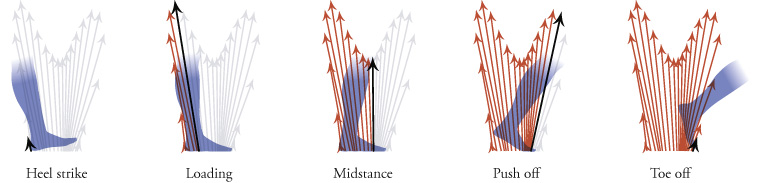
\includegraphics[width=1.0\linewidth]{chap2/2_6}
	\caption{以 1.55 米/秒的速度行走时,足部受到的典型地面反作用力。
		此处显示的力矢量(在空间中)与图~\ref{fig:2_4}~中显示的力矢量(随时间变化)相同。 \label{fig:2_6}}
\end{figure}


在站立的前半段,水平地面反作用力指向身体后部,使重心减速,之后指向身体前部。
除了图~\ref{fig:2_4}~所示的前后分量外,水平地面反作用力还有一个内外分量,这个分量虽然很小,但对于控制左右平衡很重要。
虽然在任何特定时刻重心都可能加速,但在几步匀速行走中,平均前后加速度为零。
改变前进速度时,平均前后加速度将不为零。
在垂直方向上,改变坡度时会出现非零平均加速度,例如从平地走到斜坡上时。


请记住,在步态周期的某些阶段,双脚都会接触地面,两个力相加,形成作用于身体的净向上力(图~\ref{fig:2_5})。
一个地面反作用力指向上方和前方,另一个指向上方和后方。
净地面反作用力主要指向上方,在双脚支撑阶段开始时有一个较小的向前分量,在脚趾离地时有一个较小的向后分量。
这些力抵消了向下的重力,并帮助您调节步行速度。


可以将测力板记录除以身体总质量,以估算质心加速度(公式~\ref{eq:2_2}~中的 $a_{com}$)。
该加速度可以积分一次以估算质心速度 ($v_{\text{com}}$),积分两次以估算其位置 ($r_{com}$)。
根据这些量,可以估算出质心向前的动能 ($E_{kf}$),其公式如下:
\begin{equation}
	E_{kf} = \frac{1}{2} m v_{\text{com}}
		   = \frac{1}{2} m 
		   	 ( \int a_{\text{com},f} (t) dt )^2  \label{eq:2_3}
\end{equation}
%
其中“$f$”下标表示前向分量
(请注意,垂直方向的速度波动非常小,因此我们在此忽略它)。
公式~\ref{fig:2_3}~中的积分符号提醒我们,加速度的影响是累积的,如果我们想要知道速度或动能,就必须将其随时间积分。
前向动能在站立中期最低,因为在站立的前半段,水平地面反作用力向后,使重心减速。
重力势能可以估算为:
\begin{equation}
	E_{\text{pg}} 
		= m g r_{\text{com},\text{v}} \label{eq:2_4}
\end{equation}
%
其中“v”下标表示垂直分量。
重力势能在站立中期达到最高,此时身体跨过站立肢(图 2.7)。
如果我们绘制步态周期中的前向动能和重力势能,我们会发现它们是异相的(图 2.8):
当重力势能接近最小值时,前向动能达到峰值,反之亦然。
因此,总能量几乎保持不变。
我们在行走过程中保存能量的方法之一是用重力势能换取前向动能或前向速度,类似于在重力影响下摆动的钟摆的情况。
这一观察结果表明重力与行走有很大关系。


\section{弹道步行模型}

1980年,托马斯·麦克马洪(Thomas McMahon)和西蒙$\cdot$莫雄(Simon Mochon)基于以下假设,开发了一个行走数学模型:身体将势能转化为动能,并最大限度地减少肌肉在摆动阶段的作用。
该模型非常简单,仅由三个刚性连杆和三个旋转(销)关节组成,值得注意的是,没有肌肉或运动(图2.9)。
支撑肢由一个倒立摆表示,该摆的踝关节固定在地面上,使肢体能够在矢状面上绕踝关节旋转;
支撑肢的膝盖被假设锁定在完全伸展的位置。
摆动肢被建模为一个双摆,大腿和小腿部分在膝盖处通过销连接。
两条腿在臀部处固定在一起,并具有真实的质量分布。
头部、手臂和躯干的质量被忽略,但它们的质量集中在臀部。


肌肉活动的实验记录表明,在正常速度行走过程中,除了在摆动期的开始和结束时,摆动肢的肌肉相对不活跃。
因此,弹道步行模型假设肌肉完全被动地确定模型启动和完成摆动期所需的肢体节段的位置和速度,仅受重力作用(就像抛射物,因此称为“弹道”)。
当肌肉不活跃时,摆动肢的行为被认为类似于非受迫双摆。
如果在脚趾离地时为模型提供恰到好处的初始条件,则摆动肢的脚趾将在摆动中期离开地面,并且膝盖将在脚接触时完全伸展。


\section{弗鲁德数}

倒立摆本身是一个比弹道行走模型更简单的模型,它无法准确预测人类的步行速度,但确实提供了一些关于人类步行速度的物理限制的重要见解。
考虑一个倒立摆,如图 2.9 左侧所示,长度为 $l$,体重 $m$ 集中在臀部。
当臀部处于最大高度时,其瞬时速度 $v$ 水平方向,踝关节的垂直反作用力 ($F$) 等于向心力:
%
\begin{equation}
	F = \frac{m v^2}{l}
\end{equation}
% 
向心力是必须施加在摆锤上,以防止其离开地面的向下力。
由于地面无法对脚施加向下的力(除非你踩到胶水),所以向心力必须由体重 $mg$ 产生。
将这些力相等,并解出速度,我们发现倒立摆模型的最大行走速度 ($v_{max}$) 为
%
\begin{equation}
	v_{\text{max}} = \sqrt{g l}
\end{equation}

我们用$v_{max}$来定义无量纲步行速度($v^{*}$):
\begin{equation}
	v_{*} = \frac{v}{v_{max}}
\end{equation}
%
当速度超过 $v_{max}$ 时,脚会离开地面;因此,$0 \leq v^{*} \leq 1$,此时我们行走时就像一个倒立摆。
弗劳德数 ($F_r$) 是一个无量纲量,表示向心力与重力之间的比率:
%
\begin{equation}
	F_r = \frac{v^2}{g l}
		= (v^{*})^2
\end{equation}













